%----------------------------------------------------------------------------
% Start
%----------------------------------------------------------------------------

\documentclass{article}

\usepackage{graphicx} % Required for the inclusion of images 
\usepackage{tocloft}
\usepackage[nottoc,numbib]{tocbibind} % Reference in TOC and numbered 
\usepackage{url} % References include URLs
\usepackage{mathtools} %Math stuff

\renewcommand{\cftsecleader}{\cftdotfill{\cftdotsep}} 
\renewcommand{\labelenumi}{\alph{enumi}.}

\setlength\parindent{0pt} % Removes all indentation from paragraphs


%----------------------------------------------------------------------------
% Document Information
%----------------------------------------------------------------------------

\begin{document}

\title{Giguesaur: Game Logic}
\author{Ashley Manson}
\date{\today}

\begin{titlepage}

\maketitle

\begin{center}
\large 
Co-Workers: Joshua La Pine \& Shahne Rodgers\\
Supervisors: Geoff Wyvill \& David Eyers\\

\vspace*{1\baselineskip} % Skip a line

Dept. of Computer Science\\
University of Otago

\end{center}

\end{titlepage}

%----------------------------------------------------------------------------
% Table of Contents
%----------------------------------------------------------------------------

\tableofcontents
\newpage

%----------------------------------------------------------------------------
% Introduction
%----------------------------------------------------------------------------

\section{Introduction}

Our vision for our completed Giguesaur application was allowing a classroom of
children, each with their their own iPad, to run around and solve a jigsaw
puzzle together. Imagine a classroom full of kids where they are all trying to
work on a single conventional jigsaw puzzle; such a scheme is in no way
pratical. The main goal of our project, besides all the design and technical
subgoals, was simply to make an application that is fun for children to play and
work together.

% Overview of the project
\subsection{Overview}
The Giguesaur application development was divided into three different
components. Joshua La Pine was in charge of developing the computer vsion part
of the project, which allows for the puzzle pieces to be rendered over top the
`game board' in the real world. Shahne Rodgers took charge of the networking
component of the project, which was crucial in allowing more than one player to
interact with the jigsaw puzzle. Finally my part of the project was to develop
the game logic and render the game to the iPad's screen.

% Background including what a puzzle is and other games
\subsection{Background}
There are many jigsaw puzzle games that are available for iOS and other
hand-held devices, such as Magic Jigsaw Puzzles \cite{ref:MagicJigsaw} and
Jigsaw Puzzle \cite{ref:JigsawPuzzle}, but the majority of them are limited in
the way they look due to them using an orthographic projection to render the
jigsaw puzzles. What this projection means is that the puzzle pieces of the
jigsaw puzzle are flat on the screen, the player can only look at the jigsaw
puzzle from top down, there is no depth and all the puzzle pieces are displayed
as the same size. This is something that does not work for the Giguesaur project
as the puzzle pieces are rendered in a perspective projection, so when the
jigsaw puzzle is rendered onto the game board it looks more realistic, as puzzle
pieces that are further away from the camera are shown to be smaller than pieces
that are closer to the camera. Another limitation of jigsaw puzzle games is the
way they can be interacted with, by which I mean the way they can be solved. The
puzzle pieces have to be placed into a predefined grid. Farms And Animals
Puzzles \cite{ref:FarmPuzzle} is an example of a game that has this grid layout
for the puzzle pieces to be placed in, which is shown in figure
\ref{fig:FarmsAnimals}, it also shows the limited orthographic perspective of
the game. The grid means that all the puzzle pieces will be placed in the centre
of the screen. This is something that was illogical for the project and I did
not want to limit the scope of the game. I have made it possible for the jigsaw
puzzle to be solved anywhere on the board, be it in the centre of the game board
or off in a corner of the game board. I also believe that it makes for a more
interesting game.

\begin{figure}[ht]
\begin{center}
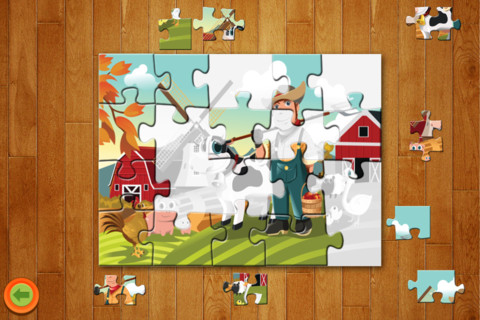
\includegraphics[width=0.85\textwidth]{images/FarmAnimalsJigsawImage}
\caption{Screenshot of Farms And Animals Puzzles \cite{img:FarmPuzzle}.}
\label{fig:FarmsAnimals}
\end{center}
\end{figure}

% iOS compared to Android
\subsection{iOS and Android}
iOS is a phone operating system made for Apples small number of hand held
devices, which are similar in many ways such as hardware and software
implementaions. Android on the otherhand is an open source operating system
based on linux of which is ran on a large number of devices crossing multiple
different versions of the operating system. The devices that Android are ran on
vary with a wide range of screen resoultions and processing power. We had
decided that the Gigusaur game would be developed for iOS for a couple of
reasons. iOS hardware was more standardized than Android, as Apple are the only
developers of iPhones and iPads it made it easy for us to write the code,
knowing that we would be relativly safe that what we developed would work on the
majority of iOS devices, at least the ones with cameras. We couldn't be certain
that any Android development of an application would work, nor would it have
been possible for a forth year project to ensure that the application would have
worked on all kinds of different Android devices. Apple also have a powerful and
intuitive integrated development environemnt (IDE) called XCode, that made
development of the Giguesaur application very easy, with its detailed profiling
tools and other features such as interface builders, it made it easier for us to
develop and quickly prototype our ideas for the application.

% Brief explaination of AR and examples
\subsection{Augmented Reality}
Augmented reality is the idea of superimposing virtural objects on top of the
real world in a realistic way that looks convincing enough for someone to
believe what they are seeing is actually physically real. In figure
\ref{fig:ARDefender} it shows a game world being played on a simple coffee
table. The game is a simple tower defence game where the user aims where the
tower shoots by moving the iPhone around the table while the camera has a marker
on the table in view. The marker on the table, of which is hidden under the
projection of the defence tower, is what allows the game to get the required
information to correctly pose the game objects onto the table. The idea of
augmented reality is what we based the Giguesaur game on, using marker trackers
to correctly pose the puzzle pieces onto the `game board' so it gives the idea
that we are interacting with jigsaw puzzle pieces in the real world.

\begin{figure}[ht]
\begin{center}
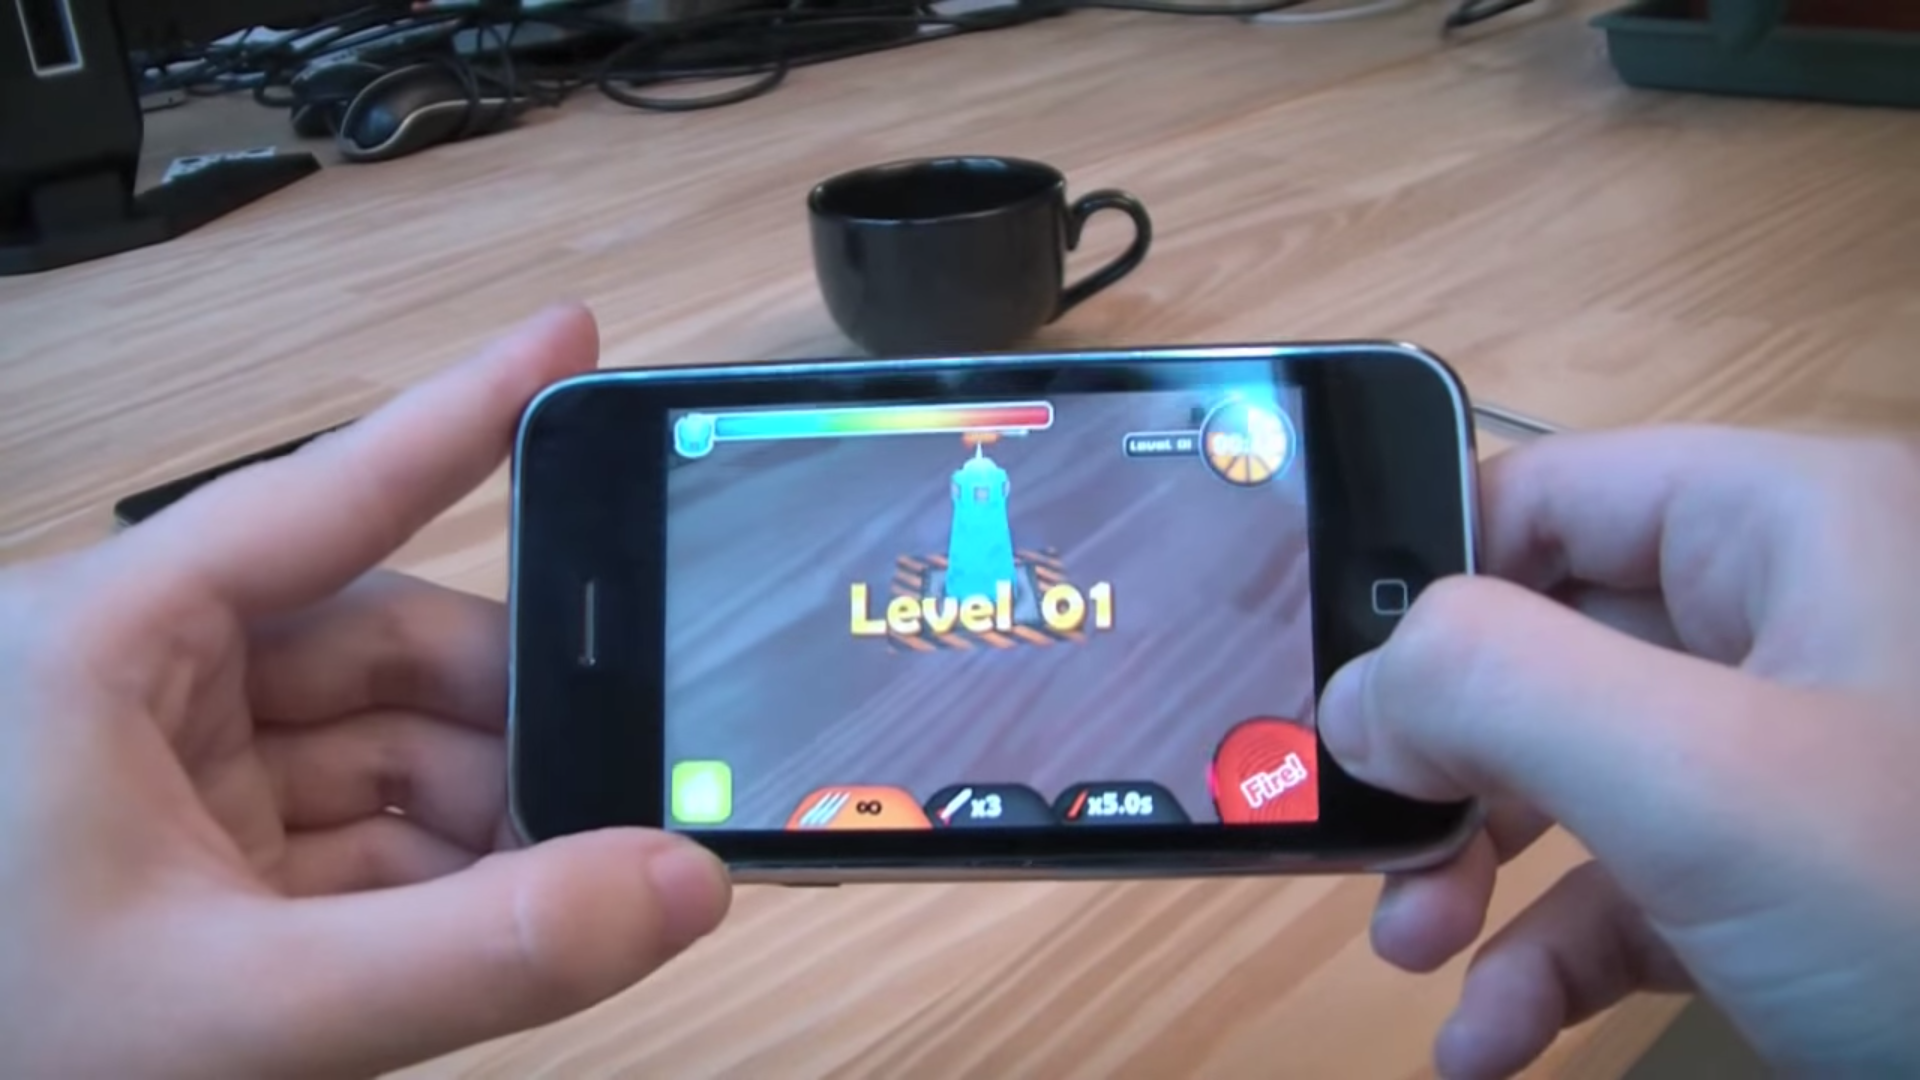
\includegraphics[width=0.85\textwidth]{images/ARDefenderImage}
\caption{Screenshot of ARDefender \cite{img:ARDefender}.}
\label{fig:ARDefender}
\end{center}
\end{figure}

% Brief introduction on my work
\subsection{Game Logic}
As I stated previously, I was in charge of developing the game logic for the
Giguesaur game. This meant I had to create the logic for how jigsaw puzzle
pieces interacted with each other and how the user interacted with the game. The
jigsaw puzzle is made up of a grid with a specific number of rows and
columns. Each piece has four edges, and an edge either has a neighbouring piece
or not. An edge of a piece can be open, meaning it has not joined to its
neighbour currently or closed meaning it has joined to its neighbour currently,
or if the edge has no neighbour it is invalid, meaning it can't join or be
joined to another piece for that edge. An invalid edge would be the outside edge
of the puzzle. Each piece of the puzzle has a unique ID, a position in space, or
an x, y coordinate on the board, and a rotation with a value between 0 and 360
degrees. The z coordinate is assumed to be 0, so it is ignored. This is how I
developed the game logic. I made up my own data structure to store these
details, the ID determines the index of the array of pieces where the piece is
held, the x, y coordinate determines where on the board the piece is displayed
and the rotation affects the orientation of the piece. The board that the pieces
are placed on has a width and length, which are along the x, y axis, which
confines where the puzzle pieces can be placed, as all the pieces have an x, y
coordinate.

%---------------------------------------------------------------------------
% Achievements
%---------------------------------------------------------------------------

\section{Achievements}

% Work done on Mac
\subsection{Prototype}
In the beginning of the project I proceded to develop a prototype of the
Giguesaur game on the Mac, using some simple OpenGL routines to render the
game. Working on the Mac helped when I was creating the game logic for the
application, as I could quickly test my ideas for the game logic such as jigsaw
puzzle piece interaction. It also allowed me to quickly try out ideas that would
be time consuming on an iPad. What I achieved with the prototype is the
following; It allowed me to get to grips with OpenGL, such as calling all the
drawing routines and getting to grips with the coordinate system, I completed
and implemented all the game mechanics for the game, such as picking up and
dropping pieces and the snapping of pieces, and I also tested out using a
perspective projection to render the game in a proper perspective. Figure
\ref{fig:MacBuild} shows what the game looks like with a perspective
projection. The broken up picture of the puppy \cite{img:OpenGLPuppy} represents
the jigsaw puzzle pieces, the green background represents the game board the
pieces are places on, and the white boarders on the edge of the game board is
the `out of bounds' area of the game board, where the pieces could not be
placed. It shows off the mechanic of pieces being snapped together, as some of
the jigsaw puzzle has been put together to be solved.

\begin{figure}[ht]
\begin{center}
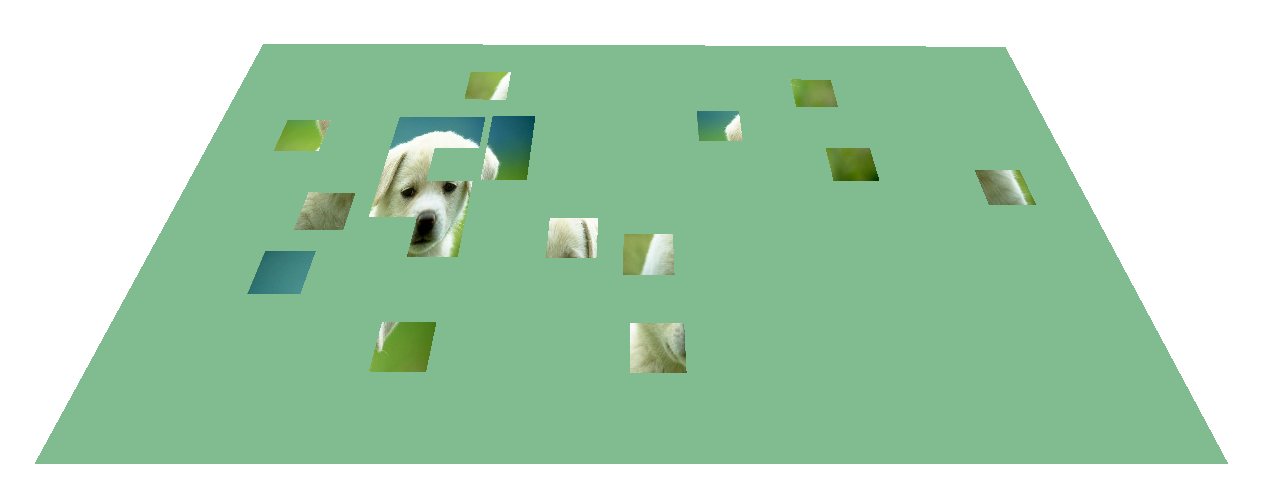
\includegraphics[width=1\textwidth]{images/MacBuildImage}
\caption{Screenshot of a prototype build on the Mac.}
\label{fig:MacBuild}
\end{center}
\end{figure}

% What the game can do
\subsection{Game Mechanics}

% The logic for piece snapping
\subsubsection{Snapping Pieces}
I wanted to enable a feature that allowed pieces to snap together, meaning if a
piece was in a specified range to its neighbour, the piece being placed back on
the board would move so that the two pieces were right next to each other, or
they snapped together, which is shown in the Java Jigsaw Puzzle game made by
Centurio \cite{ref:SourceJigsaw}. This also has the added bonus of making it
easier to check if pieces are right next to each other, rather than relying on
the user to carefully place pieces together. How the check is made to see if two
pieces should snap together is by comparing the distances between the
corresponding corner points, and if the distances are less than the snap
variable, the pieces snap together. So if the piece being put back on the board
is being snapped to its left neighbour piece, the original piece top left point
and the neighbours top right point would be checked, as well as the original
piece bottom left point and the neighbour's bottom right point would be
checked. The reason two distances are checked is to make sure that piece
rotations are taken into consideration when snapping pieces together, so as to
avoid an unusual snap where a piece rotated 90 degrees snaps to its neighbour
not rotated. When a piece is snapped to another piece, the piece saves the
rotation of its neighbour as its own, so that when the change is rendered, they
both have the same rotation when beside each other. For a puzzle to be
considered solved, all the pieces should be snapped to their corresponding
neighbours. Once a piece has snapped to its neighbour, a variable for that edge
is set as closed, as well as the neighbour's edge. So if a piece has snapped to
its right neighbour, its right edge is set as closed and the neighbour's left
edge is set as closed. The check to see if the puzzle has been solved goes
through all the pieces' edges to see if they are all closed.

% How piece rotations are handled
\subsubsection{Piece Rotations}
Each piece has an x, y coordinate location which defines where on the game board
the pieces is rendered, they also have a rotation variable that defines how the
piece is oriented on the game board. The rotation is around the z axis, where
the z axis is pointing out from the screen. The addition of rotation for puzzle
pieces added some complications to the logic of the game, in particular how I
calculated the distance between pieces for snapping as well as rendering the
pieces on screen with the correct rotations. Originally when I calculated the
distance between pieces I had been doing a simple check to see if the pieces
corner coordinates plus the length of a piece was in the range of the corner
coordinates of its neighbour. This worked fine but failed to work when piece
rotation were added, as adding the side length to the cordinates did not take
into consideration the rotation. In a replacement to this, I know calculate the
distance between piece corners using Euclidean distance, as with this I do not
have to think about the rotations of the pieces as the calulation will return
the correct values. To apply the rotation to the piece itself I use the
following simple formular:

\begin{equation*}
\begin{aligned}
x' = \cos(\theta) \times (x - x\_cen) - \sin(\theta) \times (y - y\_cen) + x\_cen\\ 
y' = \sin(\theta) \times (x - x\_cen) + \cos(\theta) \times (y - y\_cen) + y\_cen
\end{aligned}
\end{equation*}

Where $x$ and $y$ are the piece corner coordinates, $x\_cen$ and $y\_cen$ are
the piece centre coordinates, $\theta$ is the piece rotation in radians, and
$x'$ and $y'$ are the new corner cordinates. I do this for all four corners of a
piece to get the correct rotated cordinates of the piece.

% The Logic for picking up and dropping pieces
\subsubsection{Picking Up and Placing Pieces}
To pick up a piece the user taps the image of the piece on the screen. That
piece that the user has tapped is then stored in the users `inventory' and they
are no longer able to pick up another piece, until they have placed the piece
that they are holding back onto the board. The inventory is just a term I am
using to state if the user is holding or not holding a piece, meaning it can be
easily checked to see if it is empty or not. The screen x, y coordinate from a
finger tap are converted to a board x, y coordinate, z is ignored as it is
assumed to be 0. If this is close enough to a piece then that piece is added to
the user's inventory. This allows for the board to be rendered with a
perspective projection, making the scene more realistic and achieving the
augmented reality feel. When the user is holding a piece, it is moved to the
iPad centre of the screen and projected onto the board, meaning the user has to
rotate and move the iPad around to move the piece around the board. Once the
user taps the screen again, where the piece is projected on the board is where
the piece will be placed.

% Porting to iPad including changes and problems incountered
\subsection{Port to iPad}
Once I had established a working prototype for the Mac, the next step was to
port the code to an iPad. The port proved to be more difficult than I had
initially predicted. Firstly, OpenGL is handled completly differntly with iOS
than on a Mac, as it requires the use of OpenGL ES, of which I had no experience
with before. OpenGL ES is a subset of OpenGL, and it does a lot of different
things to do rendering in comparison. When using OpenGL ES with iOS, there is a
lot of set up code that goes into getting the ability to get anything to
render. Such things like getting a reference to OpenGL ES context were
required. As I had to learn the fundmentals of OpenGL ES, I based a lot of my
set up code from Wenderlich tutorial \cite{ref:RayOpenGL} on how to create an
OpenGL ES 2.0 application for iOS. Secondly, the majority of the libaries I had
written for the Mac prototype had to be re-worked and re-written to work with
iOS, as some things like data structures were not compatible across the
different environments, for example, an `NSPoint' on Mac cannot be used on iOS,
instead it is replaced with `CGPoint' and other small things like this popped up
during the port. The initial port to iOS did not have a persepctive projection,
which is shown in figure \ref{fig:iPadPort}. However, this was the first steps
into getting the application onto an iPad, and I feel like this was some serious
progress.

\begin{figure}[ht]
\begin{center}
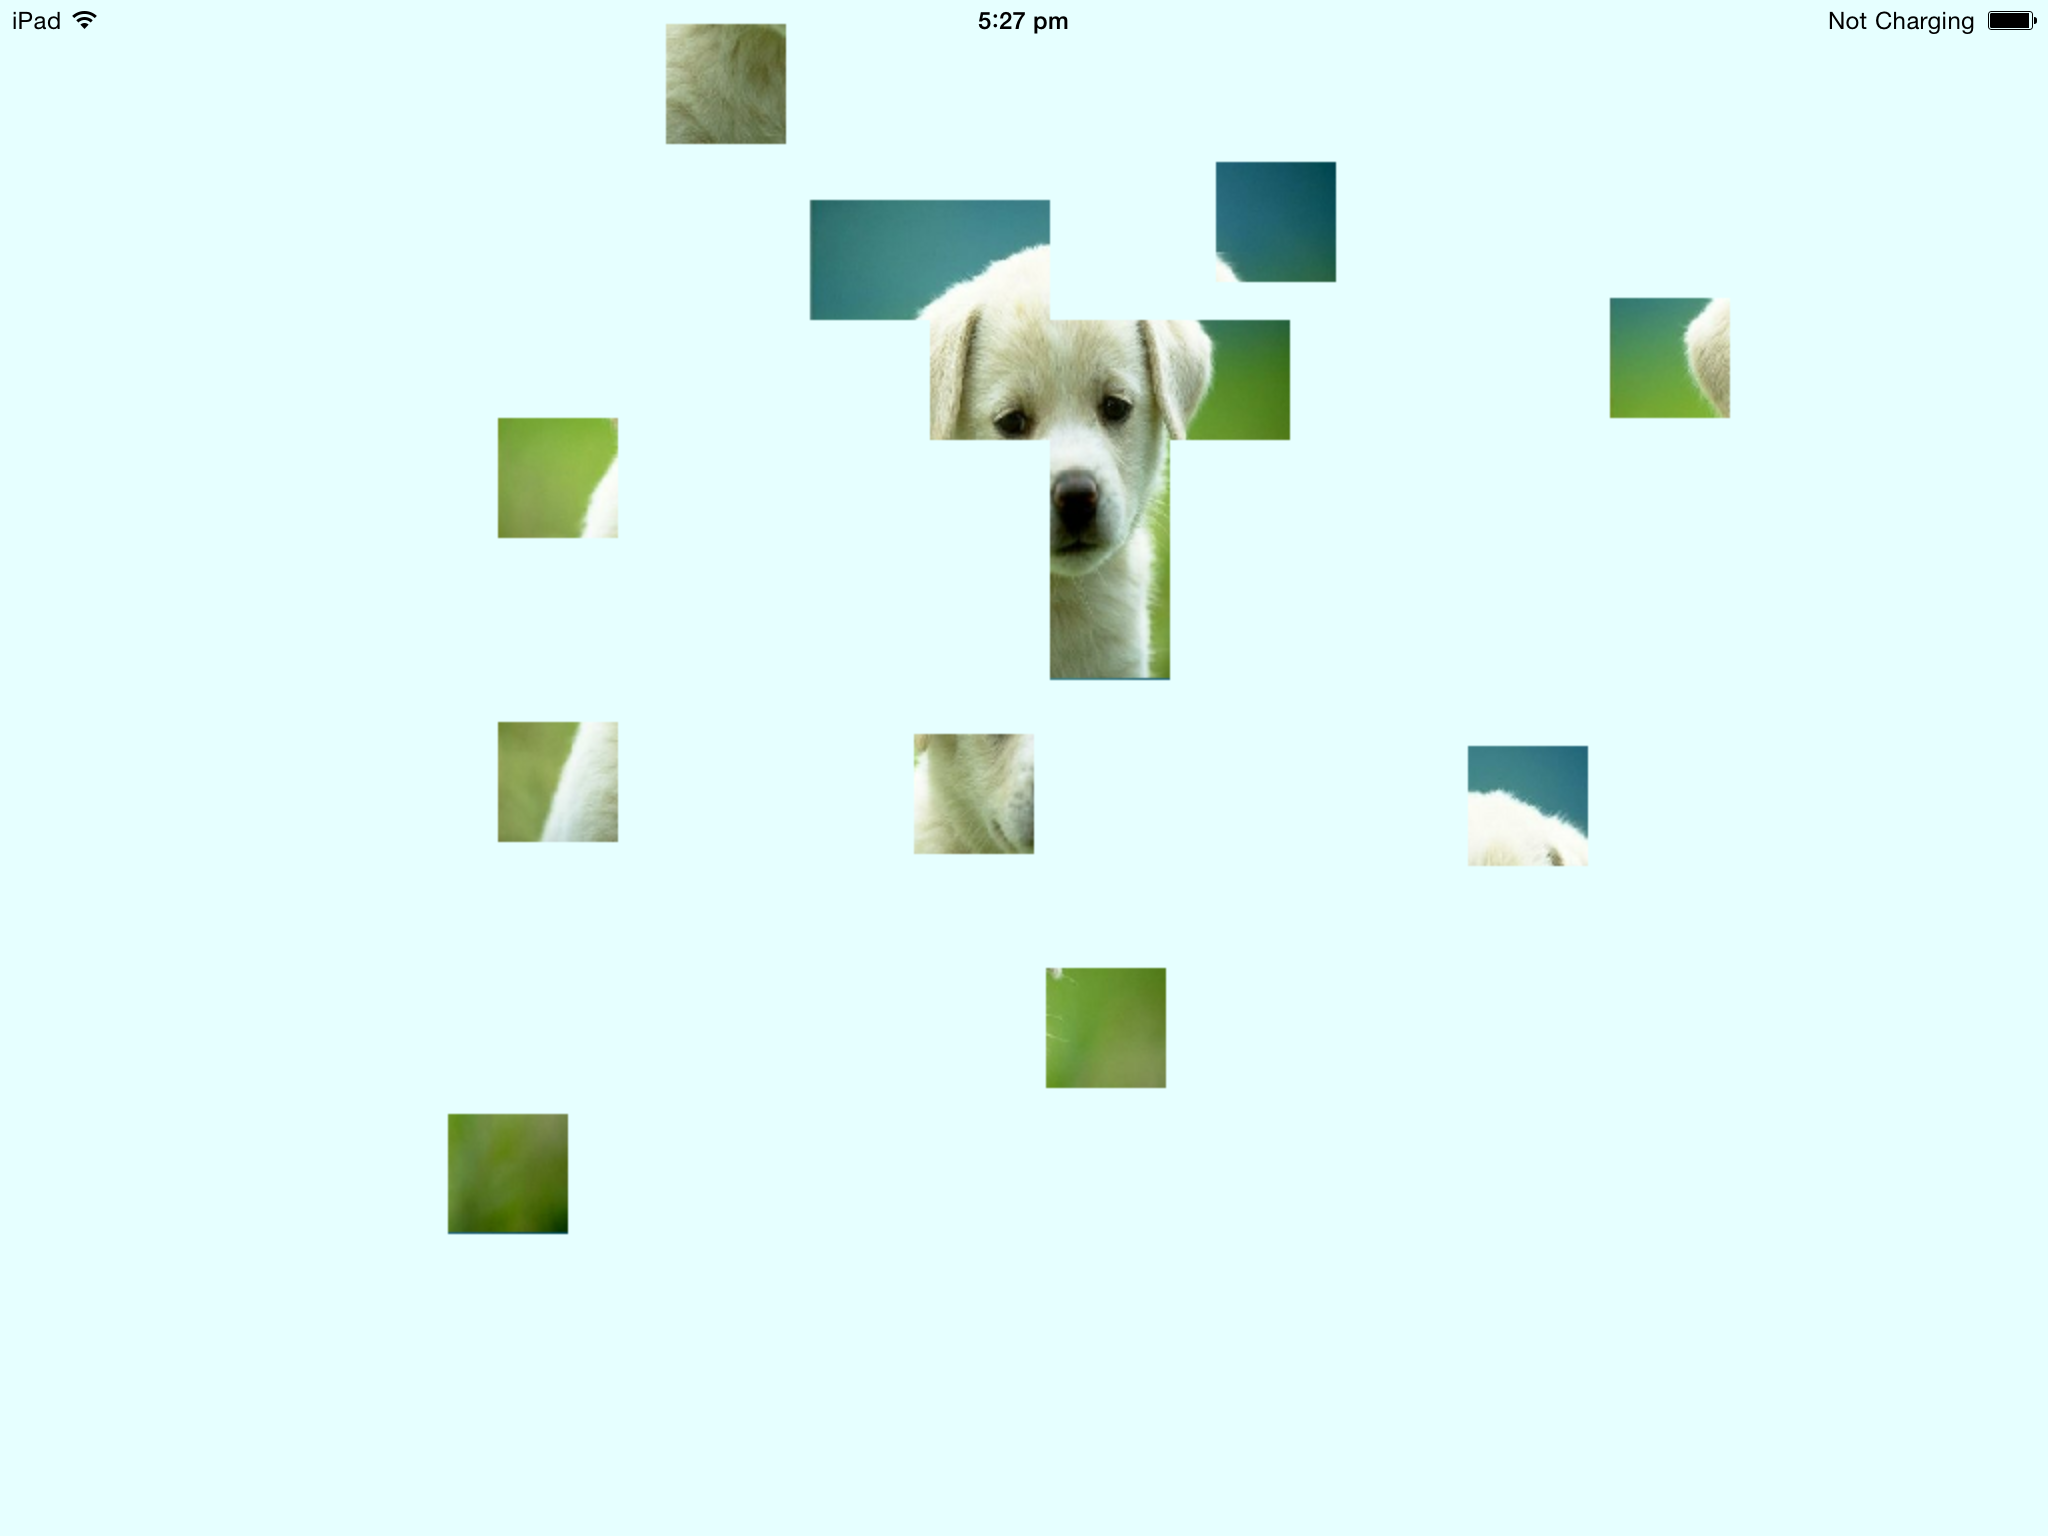
\includegraphics[width=0.85\textwidth]{images/iPadPortImage}
\caption{Screenshot of the first port to iOS.}
\label{fig:iPadPort}
\end{center}
\end{figure}

% Integrating with others including problems incountered
\subsection{Integration}
After Shahne, Josh, and I had spent the first semester working on our individual
components of the Giguesaur project, it was decided it was time to begin the
integration the three components as it was predicted this would be a difficult
process and would take some a lot of time to get everything working together. As
per the prediction, integration did take a lot of time. Not only did we have
issues of some of our code not being compatible, either by inconsisent data
types or incorrect implementations of routines, but other issues poped up such
as OpenGL and OpenCV having issues working together. There was little to no
issue with Shahne's and my part of the integration process, but on the other
hanf, Josh and I were havinf consistent trouble getting our parts working
together. It resulted in Josh and my code being closly integrated, as we had to
work together closely to get the application to properly render to the iPads'
screen. The following subsections will go into more detail for my part being
integrated with the two guys.

\subsubsection{Network and Game Logic}
For a lot of the game logic to work with the networking component, the game
logic that handled piece snapping and checking for the puzzle being solved had
to be moved into the server code. The reason for this is that all players in a
game had to be getting the same information of piece locations as everyone
else. As the piece snapping code has the chance to change the coordinates of
pieces it had to be placed in the server, so when a piece did snap, all clients
connected to the server got the updated piece location, so that it could be
reflected when the game rendered the pieces in their correct places. The code
that check for when a puzzle is solved seemed pretty logical to put it with the
server code, as when it finds that the puzzle has been solved, the server can
alert all players of this case.\\

For when a player attempts to pickup/place a piece on the game board, the client
has to ask the server if this is a legal action or not. This was a simple change
with my code to make this work, as the logic for picking up and placing pieces
will call the routines from the networking component of the code, and once the
server responds, than my code will either pickup/place a piece or take no action
based on the responce. Shahne had already prepared for this change to the code,
so this was smooth integration of our parts of the project.\\

The only issue that occured when integrating the network and game logic was that
I had stored all my piece locations as floats, while Shahne had stored the
pieces coordinates as integers, meaning that when the clients asked the server
if it was legal to place a piece in a certain place, the server would than store
the locations as integers, and update all clients of a possibly incorrect
location. This seems quite innocent at first as the lost information is quite
small, however my code that calculates piece snapping has a fractional component
as a result after it computes and an integer would lose this information which
made it insuffiecent, which shows if pieces were rotated to obscure angles, the
result would calculate a float, the server however would interpret these as
integers. The pieces than could have the possiblility to snap together
incorrectly and be offset from each other showing a visible line between
them. The fix was to refactor the integer locations into floats which took some
time.

\subsubsection{Vision and Game Logic}
The first issue we encountered when integrating the vision and game logic
components was trying to get the puzzle pieces rendered over top the video feed
coming from the camera. The issue we found here was that OpenCV was showing the
video feed on a preview layer, which was seperate from the layer that OpenGL was
rendering too. So when we attempted to get the layers to work together, either
the OpenCV layer would cover the OpenGL layer, or vice versa, meaning one layer
was always hidden from view. Something we tried was to have the OpenGL layer use
a transparent background, with the hopes that we would be able to see the video
feed behind the OpenGL layer. However, what was behind the transparent
background was just a white background which was the OpenGL default layer
colour.\\

Due to the fact it didn't seem possible to have the use of two layers
simultaneously we decided to have OpenCV create an image for each video frame,
and with each frame, send it to the OpenGL rendering code to use as the
background image for the OpenGL layer and load it in as a texture. Another issue
arised from this change, for some reason that I was unable to fix, the image
being sent from OpenCV was overriding the already loaded image for the
puzzle. So when the application first started, the picture of the puppy would
show up correctly, but as soon as the OpenCV routines kicked into gear and
started sending imaged to OpenGL, the image of the puppy seemed to disappear and
the base colour of the puzzle pieces was the only thing being rendered of the
puzzle. So we fixed one issue of not seeing what the camera could see but
introduced another problem.\\

As I could not figure out why one texture was being overridden by the other, I
decided to put trying to fix this issue on hold and move along with trying to
get the pieces showing in perspective and superimposed over the game board, as
the pieces were still showing up but with no texture on them. The issue that
arised from here the computation of the model-view matrix. What we tried to do
was have OpenCV compute the matrix so that we could use it display the puzzle
pieces in perspective. However due to either a fault in Josh's code, or mine,
the calculated model-view matrix failed to set the picesin a perspective
projection, nor would the pieces show up on screen at all. It seemed that what
ever we did to try and integrate the OpenGL with OpenCV would be meeted with
failure.\\

Due to our problems of trying to get the vision and game rendering working
together, it was decided that OpenCV would be used to render the puzzle pieces
being superimposed on the game board. For this to work, the vision code gets a
reference to the pieces array, gets and calculates the correct coordinates for
the pieces in world space, than using some simple OpenCV drawing routines, draws
the pieces over top of the game board. This allowed for not only rendering the
pieces in a correct perspective, but also solving the issue of the puzzle
textures not appearing, meaning pieces were rendering correctly. However due to
OpenGL and OpenCV having different coordinate systems, the textures of the
puzzle pieces were apperaring flipped when they were rendered to the screen,
lucklily though this was an easy fix which just required reversing the texture
coordinates of the so that they appeared correctly.\\

The different coordinate systems of OpenGL and OpenCV resulted in reverse logic
for snapping of puzzle pieces as well. As I had written my routines with the
y-axis going bottom-up as OpenGL does it, OpenCV has the y-axis going
top-down. The change to my code that I had to do to make this work was when
calculating whether a piece can snap to its up/down neighbour, reverse the
result, so when a piece would have snapped above a piece, it will now snap below
it.\\

Now the rendering the setting up of the frames is being handled by the OpenCV
routines, and my OpenGL code is being used to render the frames to the iPads
screen after each frame update. 

% Rendering of the game
\subsection{Rendering}
I was using OpenGL to do the rendering of the Mac prototype build and the
initial port to iOS, however in the final integrated application, OpenCV was
being used to create an image that is passed to the OpenGL code for it to be
rendered to the screen. The reason it is done this way is because the puzzle
piece textures have to be copied over top of the frame coming in from the
camera, which requires some extra processing to ensure the textures are shown
correctly, rather than having the puzzle pieces being rendered over the video
feed coming from the camera. Once the client recieves an image file from the
server, the OpenCV routines take the file and converts it into a OpenCV image
matrix for processing. As the main image makes up the entire puzzle texture, it
has to be split up into sections for each puzzle piece that needs to be
displayed on the game board. The number of pieces determine the number of
sections there will be as each puzzle piece will need its own section of the
texture. Than for each puzzle piece, if it is meant to be displayed currently,
the OpenCV routines will copy the associtated section of the texture to the
image frame.

%---------------------------------------------------------------------------
% Results
%---------------------------------------------------------------------------

\section{Results}
[Note: Unsure what else to add in this section]\\

We have managed to build a functional application, where multiple people can
play with the same instance of a jigsaw puzzle game, picking up and placing back
down pieces, all the while trying to solve the puzzle on screen. Figure
\ref{fig:iPadFinal} shows what the game looks like. The puzzle pieces are
rendered over top of the game board which is represented by the checkerboard,
each piece has its own rotation which is on display here. All the pieces are
simple square polygons on screen, this is due to OpenCV's limited drawing
capabilities with its drawing routines, as OpenCV can only do simple geometric
shapes. The puzzle can be solved by having all the puzzle pieces placed together
in their correct positions, the server will do a check to see if the puzzle has
been solved or not, by going through each piece in an array, checking to see if
each pieces' edge has been closed or not.

\begin{figure}[ht]
\begin{center}
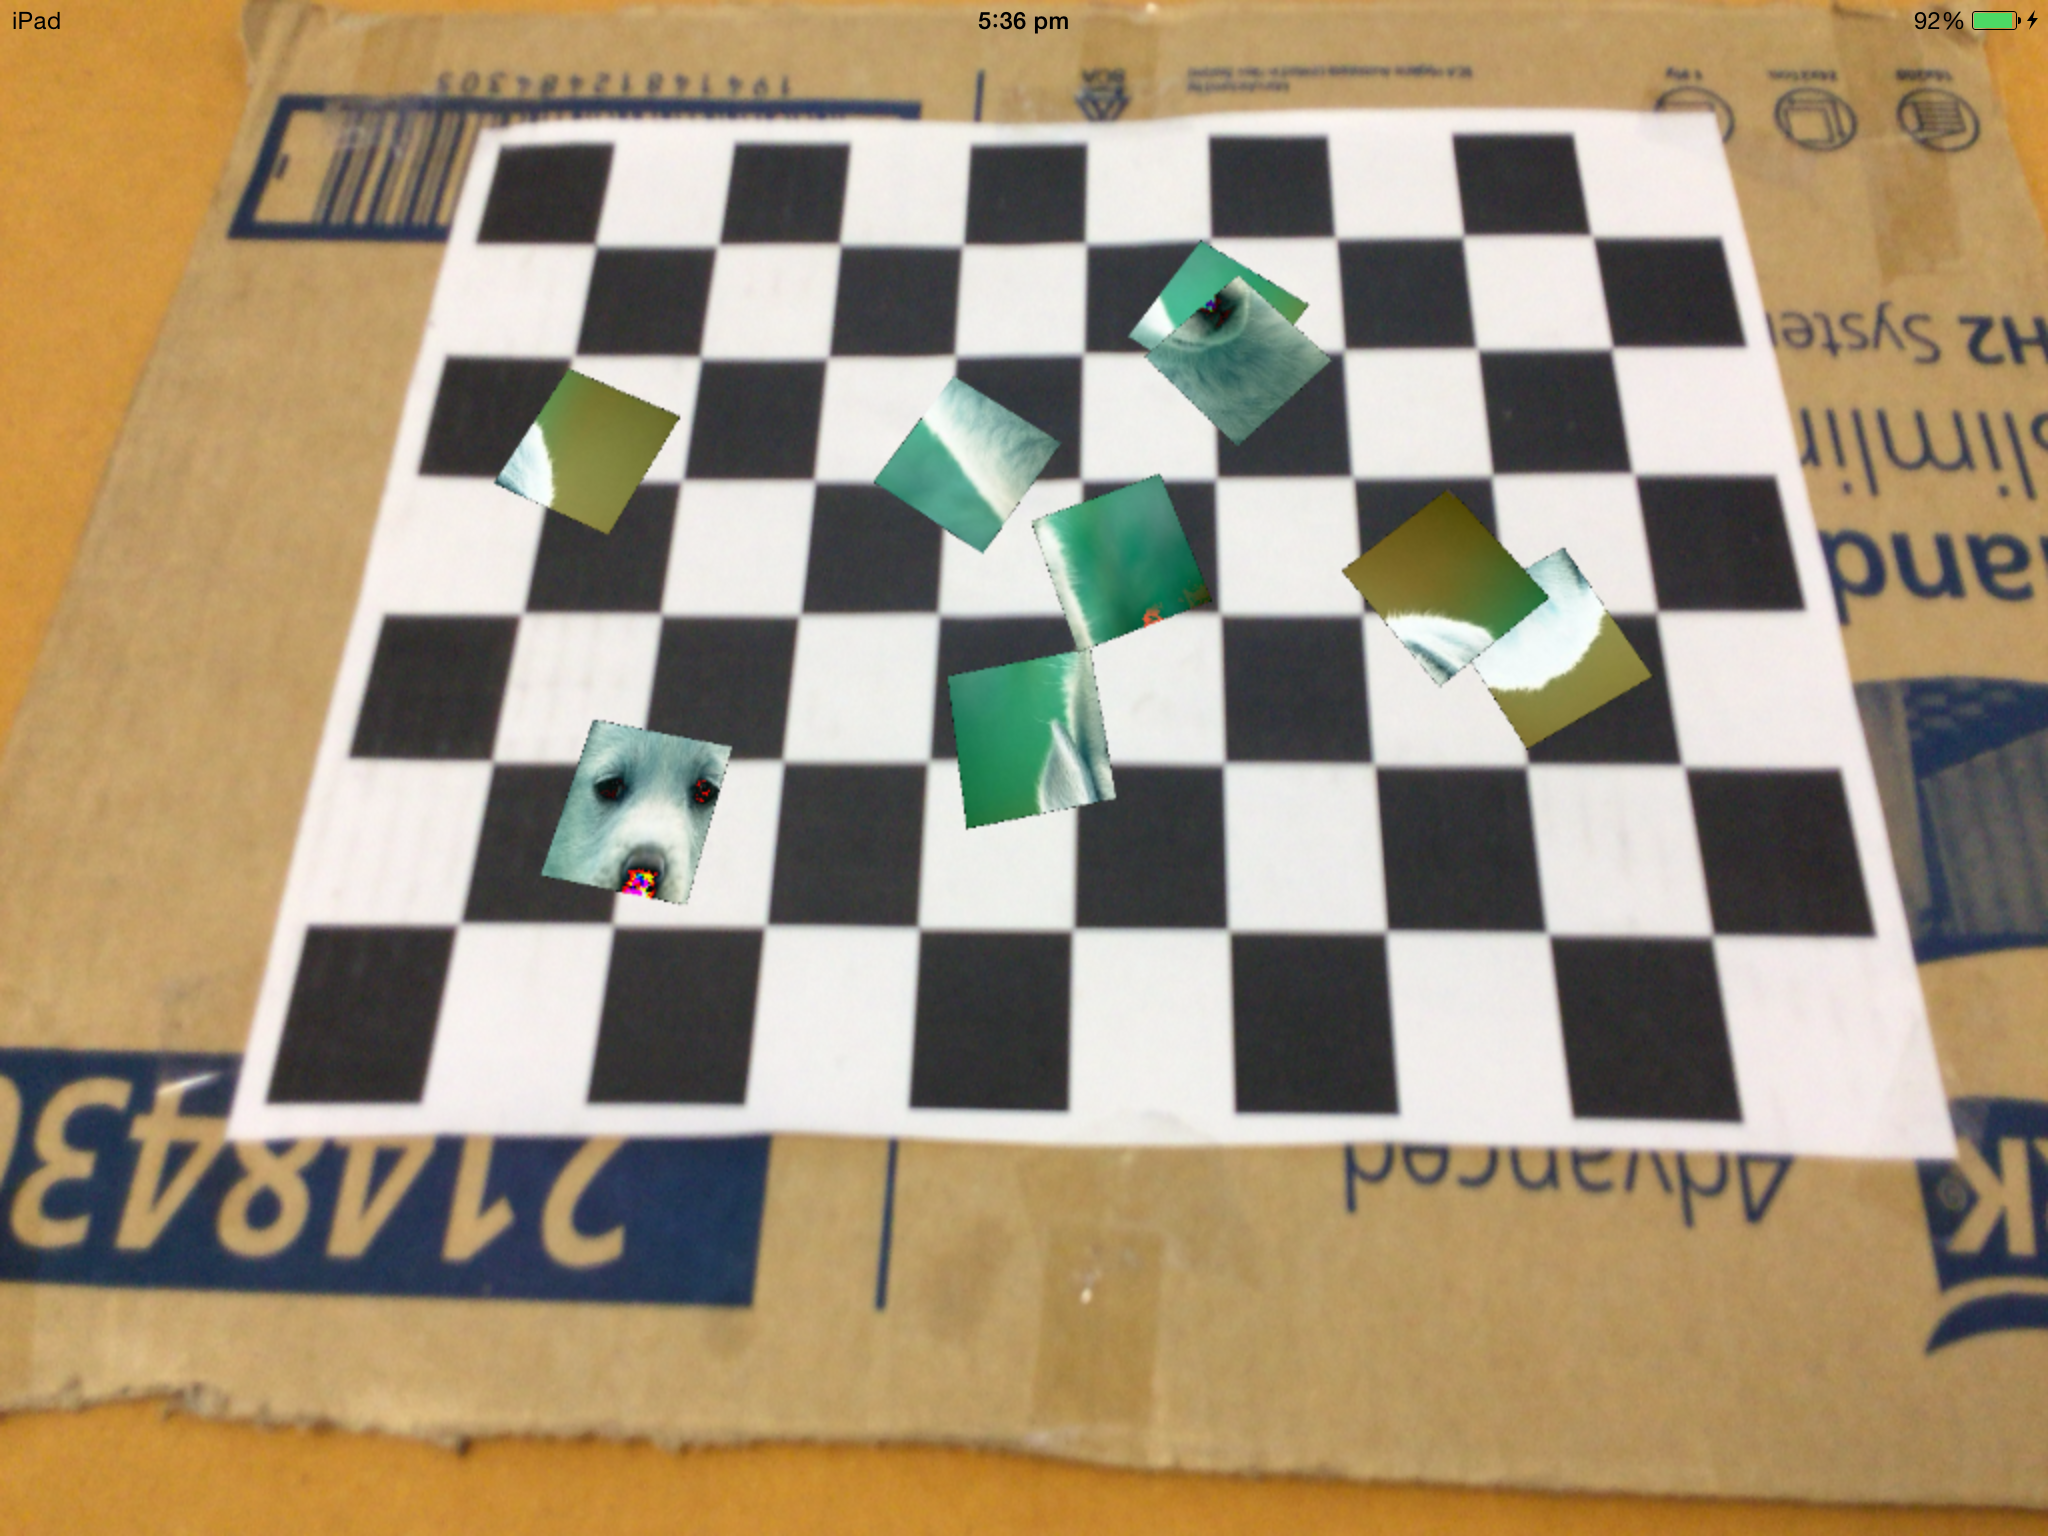
\includegraphics[width=0.85\textwidth]{images/iPadFinalImage}
\caption{Screenshot of the final build running on an iPad.}
\label{fig:iPadFinal}
\end{center}
\end{figure}

%---------------------------------------------------------------------------
% Conclusion
%---------------------------------------------------------------------------

\section{Conclusion}

% What hasn't been done
\subsection{Future Work}
[Note: I need to expand out each future work; 1. Why wasn't it done? 2. How
  could it be finished? 3. Idea for future implementations?]\\

There are still a couple things that I have missed out on implementing for the
game logic and rendering of the Giguesaur application. Firstly, puzzle pieces
are still only simple square polygons. In future, this would be changed so that
pieces have curved edges, similar to figure \ref{fig:FarmsAnimals} earlier in
the document, where you can see the curved edges of pieces. The curved edges to
pieces would not only make the game look more like jigsaw puzzle game, but it
would also allow for players to easily solve the puzzle rather than having to
match the images on the current puzzle pieces. This would be implemented using a
random number generator that would choose a certain number of points along the each pieces edge, and than map vertices along each point, Secondly, the
application is quite slow, with it only running at a maximum of five frames per
second, performing even worst than that on average. Due to the fact that the
OpenCV functions that calculate the perspective projection matrix are quite
slow.

% Final Wrap Up
\subsection{Discussion}
[Place Holder Text]

%---------------------------------------------------------------------------
% References
%---------------------------------------------------------------------------

\clearpage
\bibliographystyle{ieeetr}
\bibliography{references}

%---------------------------------------------------------------------------
% End
%---------------------------------------------------------------------------

\end{document}
